\begin{ccRefConcept}{PureComplexDataStructure}

\ccDefinition

The \ccRefName\ concept describes objects responsible for storing and
maintaining $d$-dimensional pure complexes \emph{embedded} in
$\sphere^D=\real^D\cup\{\infty\}$ that triangulate a topological sphere
$\sphere^d$ with $d\in[-2,D]$. A pure (or homogeneous) $d$-complex is a
simplicial complex all of whose simplices are faces of some $d$-simplex. (A
simplex is also a face of itself.) In particular, a pure $d$-complex does not
contain any $d+1$-simplex.

Values of $d$ (the \emph{current dimension} of the complex) include \begin{itemize}

\item[-2] This corresponds to the non-existence of any object in
$\sphere^D.$

\item[-1] This corresponds to a single vertex and a single simplex. In a
geometric realization of the \ccRefName\ (\emph{e.g.}, in a
\ccc{Pure_complex<PCTraits, PCDS>} or a
\ccc{Delaunay_complex<DCTraits, PCDS>}), this vertex
corresponds to \emph{the vertex at infinity}.

\item[0] This corresponds to two vertices, each adjacent to one $0$-simplex;
the two simplices being neighbor of each other. This is the unique
triangulation of the $0$-sphere.

\item[$d>0$] This corresponds to a standard triangulation of the sphere
$\sphere^d$.
\end{itemize}

An $i$-simplex is a simplex with $i+1$ vertices. An $i$-simplex $\sigma$ is
\textbf{incident} to a $j$-simplex $\sigma'$, $j<i$, if and only if $\sigma'$
is a proper face of $\sigma$. Two simplices are \textbf{adjacent} if the
intersection of their vertex-set is not empty.

\ccHasModels

\ccc{Pure_complex_data_structure<Dimensionality, PCDSVertex, PCDSSimplex>}

\ccTypes

\ccNestedType{Vertex}
{
A model of the concept \ccc{PureComplexDSVertex}.
}
\ccGlue
\ccNestedType{Simplex}
{
A model of the concept \ccc{PureComplexDSSimplex}.
}

The concept \ccRefName\ also defines a type for describing facets of the
pure complex with codimension~1:

\ccTypedef{typedef std::pair<Simplex_handle, int> Facet;}
{A facet of a (full dimensional) simplex. It is of dimension
\ccc{current_dimension()-1}. \ccc{Facet f(s,i)} represents the facet of
simplex \ccc{s} opposite to its \ccc{i}-th vertex}

\ccNestedType{Face}
{A model of the concept \ccc{PureComplexFace}.}

Vertices and simplices are manipulated via \emph{handles}. Handles support the
usual two dereference operators \ccc{operator*} and \ccc{operator->}.

\ccNestedType{Vertex_handle}
{
Handle to a \ccc{Vertex}.
}
\ccGlue
\ccNestedType{Vertex_const_handle}
{
Handle to a \ccc{const Vertex}.
}
\ccGlue
\ccNestedType{Simplex_handle}
{
Handle to a \ccc{Simplex}.
}
\ccGlue
\ccNestedType{Simplex_const_handle}
{
Handle to a \ccc{const Simplex}.
}

Vertices, facets and simplices can be iterated over using \emph{iterators}.
Iterators support the usual two dereference operators \ccc{operator*} and
\ccc{operator->}.

\ccNestedType{Vertex_iterator}
{
Iterator over the list of vertices.
}
\ccGlue
\ccNestedType{Vertex_const_iterator}
{
Iterator over the list of vertices (\ccc{const} casted).
}
\ccGlue
\ccNestedType{Simplex_iterator}
{
Iterator over the list of simplices.
}
\ccGlue
\ccNestedType{Simplex_const_iterator}
{
Iterator over the list of simplices (\ccc{const} casted).
}
\ccGlue
\ccNestedType{Facet_iterator}
{
Iterator over the facets of the complex.
}

\ccNestedType{size_type}{Size type (an unsigned integral type)}
\ccNestedType{difference_type}{Difference type (a signed integral type)}

\ccCreation
\ccCreationVariable{c}

\ccConstructor{PureComplex(const int dim);} { Creates an instance \ccVar\ of
type \ccRefName. The maximal dimension of its simplices is \ccc{dim} and
\ccVar\ is initialized to the empty pure complex. Thus,
\ccVar.\ccc{current_dimension()} equals \ccc{-2}.}

%\ccOperations

\ccHeading{Queries}	% --------------------------------------------- QUERIES

\ccMethod{int ambient_dimension() const;} { Returns the maximal dimension of
the simplices that can be stored in the pure complex \ccVar. \ccPostcond the
returned value is positive. }

\ccMethod{int current_dimension() const;} { Returns the dimension of the
simplices stored in the complex. It holds that
\ccVar.\ccc{current_dimension()=-2} if and only if \ccVar.\ccc{empty()} is
\ccc{true}. \ccPostcond the returned value \ccc{d} must satisfy \ccc{-2 <= d
<=}\ccVar.\ccc{ambient_dimension()}. }

\ccMethod{bool empty() const;} { Returns \ccc{true} if the regular complex
contains no simplex. Returns \ccc{false} otherwise. }

\ccMethod{size_type number_of_vertices() const;}
{Returns the number of vertices stored in the regular complex.}

\ccMethod{size_type number_of_simplices() const;}
{Returns the number of simplices stored in the regular complex.}

\ccMethod{bool is_vertex(const Vertex_const_handle & v) const;}
{}

\ccMethod{bool is_simplex(const Simplex_const_handle & s) const;}
{}

\ccMethod{template< typename TraversalPredicate, typename OutputIterator >
void gather_simplices(Simplex_handle s, TraversalPredicate & tp,
OutputIterator & out) const;}
{This function computes (\emph{gathers}) a connected set of simplices
satifying a common criteria. Call them \emph{good} simplices. It is assumed
that the argument \ccc{s} is a good simplex. The simplices are then
recursively explored by examining if, from a given good simplex, its neighbor
simplices are also good.\\
The argument \ccc{tp} is a predicate that takes as argument a \ccc{Facet}
whose containing \ccc{Simplex} is good. The predicate must return \ccc{true}
if the traversal of that \ccc{Facet} leads to a good simplex.\\
All the good simplices are outputed into the last argument \ccc{out}.}

\ccMethod{template< typename OutputIterator > OutputIterator
gather_incident_simplices(Vertex_const_handle v, OutputIterator out) const;}
{Insert in \ccc{out} all the simplices that are incident to the vertex
\ccc{v}, \emph{i.e.}, the simplices that have the \ccc{Vertex v} as a vertex.
Returns the (modified) output iterator.
\ccPrecond\ccc{is_simplex(f.simplex())}.}

\ccMethod{template< typename OutputIterator > OutputIterator
gather_incident_simplices(const Face & f, OutputIterator out) const;}
{Insert in \ccc{out} all the simplices that are incident to the face \ccc{f},
\emph{i.e.}, the simplices that have the \ccc{Face f} as a subface.
Returns the (probably modified) output iterator.
\ccPrecond\ccc{is_simplex(f.simplex())}.}

\ccMethod{template< typename OutputIterator > OutputIterator
gather_adjacent_simplices(const Face & f, OutputIterator out) const;}
{Insert in \ccc{out} all the simplices that are adjacent to the face \ccc{f},
\emph{i.e.}, the simplices that share at least one vertex with the \ccc{Face
f}. Returns the (probably modified) output iterator.
\ccPrecond\ccc{is_simplex(f.simplex())}.}

\ccMethod{template< typename OutputIterator > OutputIterator
gather_incident_faces(Vertex_const_handle v, const int d, OutputIterator
out);}{Constructs all the \ccc{Face}s of dimension \ccc{d} incident to
\ccc{Vertex} v and inserts them in the \ccc{OutputIterator out}.  If \ccc{d
>=} \ccVar.\ccc{current_dimension()}, then no \ccc{Face} is
constructed.\ccPrecond\ccc{0 < d}.}

\ccMethod{template< typename OutputIterator > OutputIterator
gather_incident_upper_faces(Vertex_const_handle v, const int d, OutputIterator
out);}{Constructs all the \textbf{upper} \ccc{Face}s of dimension \ccc{d}
incident to \ccc{Vertex} v and inserts them in the \ccc{OutputIterator out}.\\
Assuming some total ordering on the vertices of the complex (which is
invariant as long as no vertex is inserted in or removed from the complex), a
\ccc{Face} incident to \ccc{v} is an \emph{upper} \ccc{Face} if and only if
its vertices occur at \ccc{v} or beyond \ccc{v} in the ordering.\\ In
particular, taking the disjoint union of the upper \ccc{Face}s of dimension
\ccc{d} incident to every vertex of the complex yields exactly the set of
faces of dimension \ccc{d} of the complex.\\ The constructed \ccc{Faces} are
lexicographically ordered (using the vertex order as base ordering). If \ccc{d
>=} \ccVar.\ccc{current_dimension()}, then no \ccc{Face} is
constructed.\ccPrecond\ccc{0 < d}.}

\ccGlue\ccMethod{template< typename OutputIterator, typename Comparator >
OutputIterator gather_incident_upper_faces(Vertex_const_handle v, const int d,
OutputIterator out, Comparator cmp);} {Same as above, but uses \ccc{cmp} as
the vertex ordering to define the upper faces.}

\ccHeading{Accessing the vertices} % --------------------- ACCESS TO VERTICES

\ccMethod{Vertex_handle vertex(Simplex_handle s, const int i) const;}{}
\ccGlue
\ccMethod{Vertex_const_handle vertex(Simplex_const_handle s, const int
i) const;}
{ Returns a handle to the \ccc{i}-th \ccc{Vertex} of the \ccc{Simplex} \ccc{s}.
\ccPrecond \ccc{0 <= i <=} \ccVar.\ccc{current_dimension()}.}

\ccMethod{int mirror_index(Simplex_handle s, int i) const;}{}
\ccGlue\ccMethod{int mirror_index(Simplex_const_handle s, int i) const;}
{Returns the index of the vertex mirror of the \ccc{i}-th vertex of \ccc{s}.
Equivalently, returns the index of \ccc{s} in its \ccc{i}-th opposite simplex.
If there is no simplex opposite to the \ccc{i}-th vertex of \ccc{s}, then
returns \ccc{-1}. \ccPrecond \ccc{0 <= i <=} \ccVar.\ccc{current_dimension}()\\
and \ccc{s != Simplex_handle()}. }

\ccMethod{Vertex_const_iterator vertices_begin() const;}
{
}
\ccGlue
\ccMethod{Vertex_iterator vertices_begin();}
{
The first vertex of \ccVar.
}
\ccGlue
\ccMethod{Vertex_const_iterator vertices_end() const;}
{
}
\ccGlue
\ccMethod{Vertex_iterator vertices_end();}
{
The beyond vertex of \ccVar.
}

\ccHeading{Accessing the simplices} % ------------------- ACCESS TO SIMPLICES

\ccMethod{Simplex_handle simplex(Vertex_handle v) const;}{}
\ccGlue
\ccMethod{Simplex_const_handle simplex(Vertex_const_handle v) const;}
{Returns a simplex adjacent to \ccc{Vertex} \ccc{v}. Note that this simplex is
not unique (\ccc{v} is typically adjacent to more than one simplex).
\ccPrecond\ccc{v != Vertex_handle()}}

\ccMethod{Simplex_handle neighbor(Simplex_handle s, int i) const;}{}
\ccGlue
\ccMethod{Simplex_const_handle neighbor(Simplex_const_handle s, int i)
const;} { Returns a \ccc{Simplex_handle} pointing to the \ccc{Simplex}
opposite to the \ccc{i}-th vertex of \ccc{s}. If there is no opposite simplex,
then returns \ccc{Simplex_handle()}.
\ccPrecond\ccc{0 <= i <=}\ccVar.\ccc{current_dimension()}\\
and \ccc{s != Simplex_handle()}}

\ccMethod{Simplex_const_iterator simplices_begin() const;}
{
}
\ccGlue
\ccMethod{Simplex_iterator simplices_begin();}
{
The first simplex of \ccVar.
}
\ccGlue
\ccMethod{Simplex_const_iterator simplices_end() const;}
{
}
\ccGlue
\ccMethod{Simplex_iterator simplices_end();}
{
The beyond simplex of \ccVar.
}

\ccHeading{Faces and Facets} % - - - - - - - - - - - - - - - - - - - - FACETS

\ccMethod{Facet_iterator facets_begin();}
{Iterator to the first facet of the complex.}
\ccGlue
\ccMethod{Facet_iterator facets_end();}
{Iterator to the beyond facet of the complex.}

\ccMethod{Simplex_handle simplex_of(const Facet & f) const;}
{Returns a simplex containing the facet \ccc{f}}

\ccMethod{int index_of_covertex(const Facet & f) const;}
{Returns the index of vertex of the simplex \ccc{s=}\ccVar.\ccc{simplex_of(f)}
which does \textbf{not} belong to \ccc{s}.}

\ccMethod{Face make_empty_face() const;}{Returns an empty \ccc{Face}.}

\begin{ccAdvanced}

\ccMethod{bool is_boundary_facet(const Facet & f) const;}
{When a subset of the simplices has their \ccc{flags} set to \ccc{1}, this
function returns \ccc{true} when the \ccc{Facet f} is part of the boundary of
that subset, and \ccc{false} otherwise.}

\end{ccAdvanced}

\ccHeading{Vertex removal} % - - - - - - - - - - - - - - - - - - - - REMOVALS

\ccMethod{void clear();}
{Reinitializes \ccVar\ to the empty complex.}

\ccMethod{Vertex_handle contract_face(const Face & f);} {Contracts the
\ccc{Face f} to a single vertex. Returns a handle to that vertex. \ccPrecond
The contracted pure complex must be valid (\emph{i.e.}, be a triangulation of
a sphere of dimension \ccVar.\ccc{current_dimension()}).}

\ccMethod{void remove_decrease_dimension(Vertex_handle v, Vertex_handle
star);} {This method does exactly the opposite of
\ccc{insert_increase_dimension()}. \ccPrecond Both vertices \ccc{v} and
\ccc{star} must share an edge with all vertices.
\ccc{current_dimension() >= -1}.}

\begin{ccAdvanced}

\ccMethod{void delete_vertex(Vertex_handle v);}
{Remove the vertex \ccc{v} from the pure complex. This does not take care of
erasing the references to \ccc{v} in other parts of the complex!}

\ccMethod{void delete_simplex(Simplex_handle s);}
{Remove the simplex \ccc{s} from the pure complex. This does not take care of
erasing the references to \ccc{s} in other parts of the complex!}

\ccMethod{template< typename ForwardIterator > void
    delete_simplices(ForwardIterator start, ForwardIterator end);}
{Remove the simplices in the range \ccc{[start,end)} from the pure complex.
This does not take care of erasing the references to \ccc{s} in other parts of
the complex!}

\end{ccAdvanced}

\ccHeading{Vertex insertion} % - - - - - - - - - - - - - - - - - - INSERTIONS

\ccMethod{Vertex_handle insert_in_simplex(Simplex_handle s);}{Inserts a new
vertex \ccc{v} in the simplex \ccc{s} and returns a handle to it. The simplex
\ccc{s} is subdivided into \ccVar.\ccc{current_dimension())+1} simplices which
share the vertex \ccc{v}.
\ccPrecond\ccc{0 <} \ccVar.\ccc{current_dimension()}\\ and
\ccc{Simplex_handle() != s}\\ and \ccc{s} is a simplex of \ccVar.}
\begin{ccTexOnly}
\begin{center}
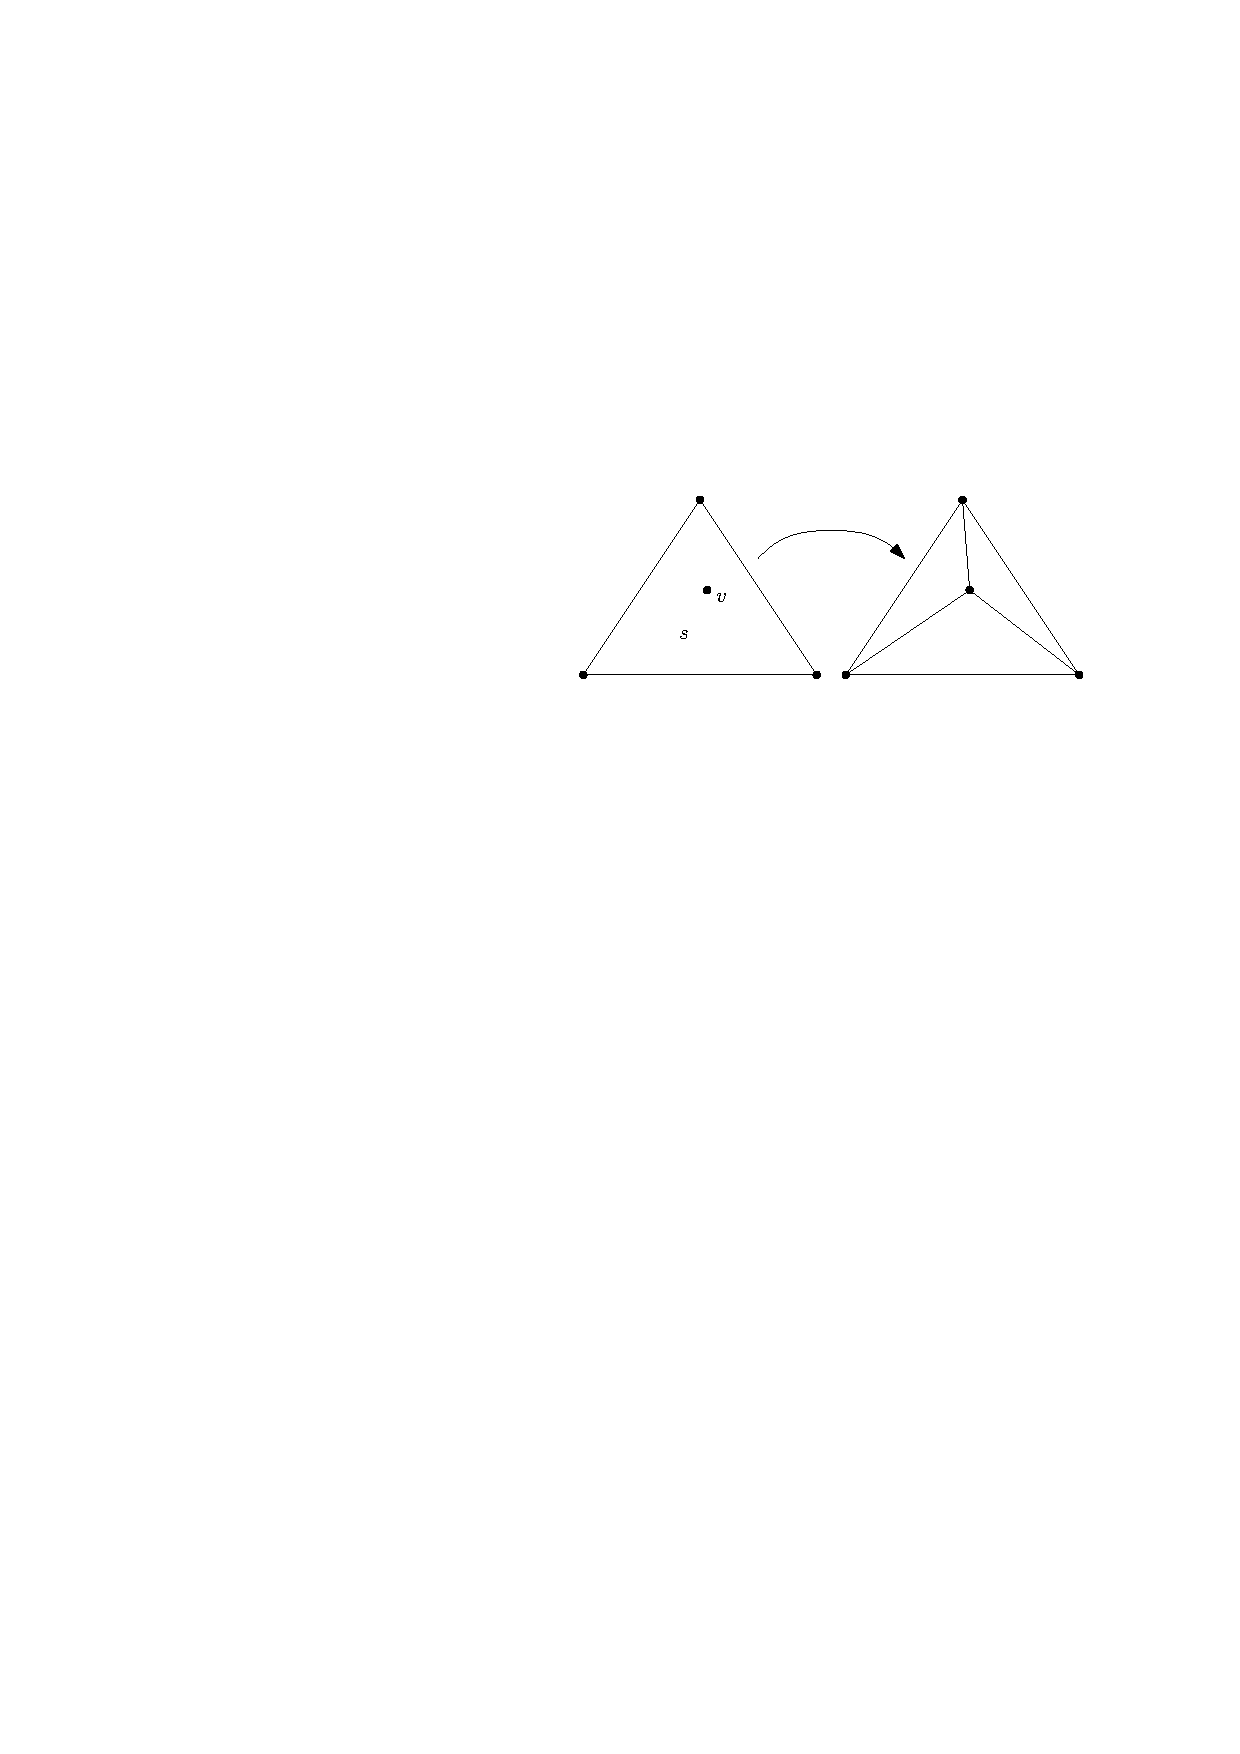
\includegraphics{Pure_complex_ref/fig/insert-in-simplex.pdf}
\end{center}
\end{ccTexOnly}
\begin{ccHtmlOnly}
<center>
<img border=0 src="./fig/insert-in-simplex.png" align="middle" alt="The effect of insert_in_simplex()">
</center>
\end{ccHtmlOnly}

\ccMethod{Vertex_handle insert_in_face(const Face & f);}
{Inserts a vertex in the pure complex data structure by subdividing the
\ccc{Face f}. Returns a handle to the newly created \ccc{Vertex}.}
\begin{ccTexOnly}
\begin{center}
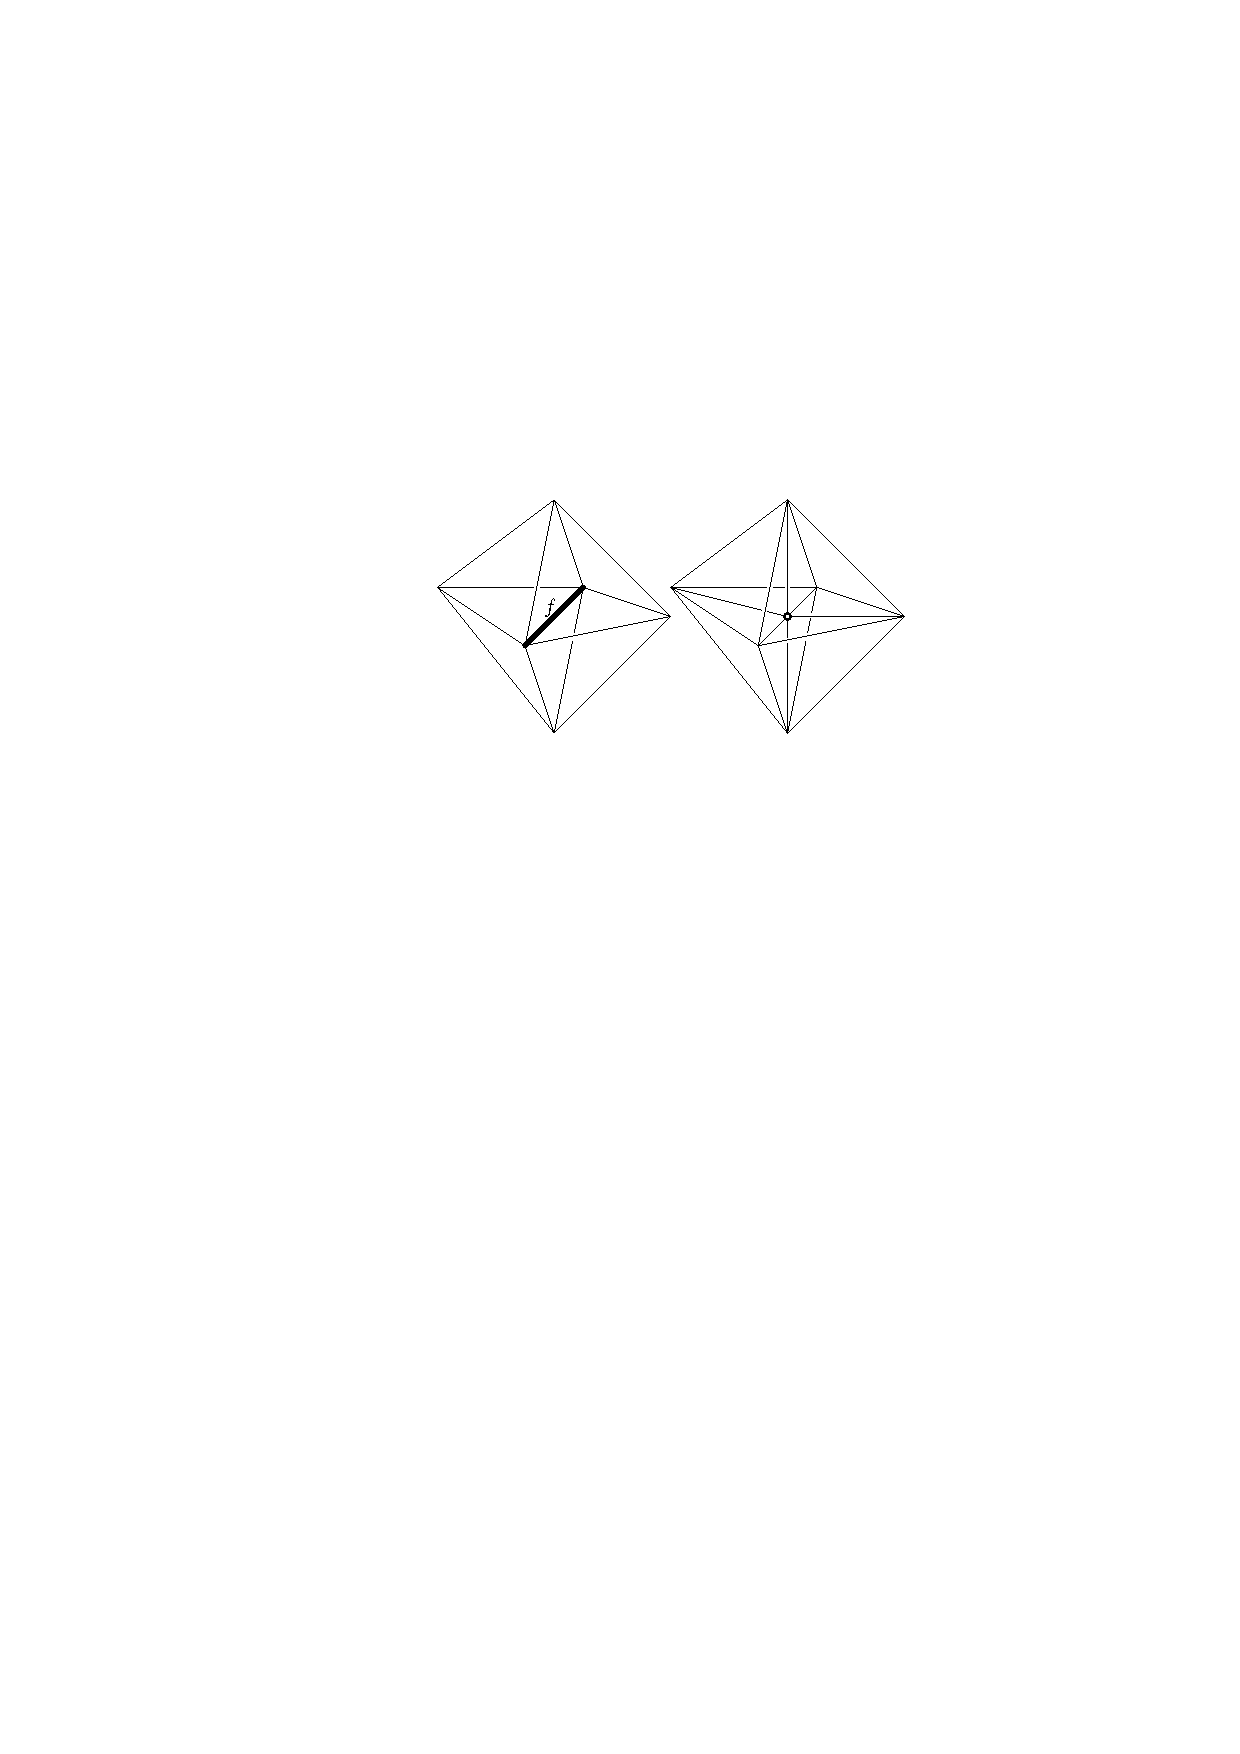
\includegraphics{Pure_complex_ref/fig/insert-in-face.pdf}
\end{center}
\end{ccTexOnly}
\begin{ccHtmlOnly}
<center>
<img border=0 src="./fig/insert-in-face.png" align="middle" alt="The effect of insert_in_face()">
</center>
\end{ccHtmlOnly}

\ccMethod{Vertex_handle insert_in_facet(const Facet & ft);}
{Inserts a vertex in the pure complex data structure by subdividing the
\ccc{Facet ft}. Returns a handle to the newly created \ccc{Vertex}.}

\ccMethod{template< class ForwardIterator > Vertex_handle
insert_in_hole(ForwardIterator start, ForwardIterator end, Facet f);}{The
simplices in the range \ccc{C=[start, end)} are removed, thus forming a hole.
A \ccc{Vertex} is inserted and connected to the boundary of the hole in order
to ``close it''. A \ccc{Vertex_handle} to the new \ccc{Vertex} is returned.
\ccPrecond \ccc{C} must be a (combinatorial) ball and not contain any vertex
all of whose adjacent simplices are in \ccc{C}. (This implies that
\ccVar.\ccc{current_dimension() >= 2} if \ccc{|C|>1}.)\\ The boundary of
\ccc{C} must be a (combinatorial) triangulation of the sphere
$\sphere^{d-1}$.}
\ccGlue
\ccMethod{template< class ForwardIterator, class OutputIterator >
Vertex_handle insert_in_hole(ForwardIterator start, ForwardIterator end, Facet
f, OutputIterator out);}{Same as above, but handles to the new simplices are
appended to the \ccc{out} output iterator.}

\ccMethod{Vertex_handle insert_increase_dimension(Vertex_handle star);}
{Transforms a complex that triangulates the sphere $\sphere^d$ into the
triangulation of the sphere $\sphere^{d+1}$ by adding a new vertex \ccc{v}:
\ccc{v} is added to all simplices that do not contain the vertex \ccc{star} so
as to triangulate one of the two half-spheres of $\sphere^{d+1}$. The vertex
\ccc{star} already does triangulate the second half-sphere. (When there is an
associated geometric triangulation, \ccc{star} is in fact the vertex
associated with its infinite vertex.) The storage of the vertices in the
simplices is such that, if \ccc{f} was a simplex of maximal dimension in the
initial complex, then \ccc{(f,v)}, in this order, is the corresponding simplex
in the updated complex. A handle to \ccc{v} is returned.
\ccPrecond\ccVar.\ccc{current_dimension() < }
\ccVar.\ccc{ambient_dimension()}\\ and \ccc{is_vertex(star)}}

\begin{ccAdvanced}

The following methods may destroy the integrity (the ``purity'', one may say)
of the data structure. They are used internally. Use at your own risks.

\ccMethod{Simplex_handle new_simplex();} {Adds a new simplex to \ccVar\ and
returns a handle to it. The new simplex has no vertex and no neighbor yet.}

\ccMethod{Vertex_handle new_vertex();}
{Adds a new vertex to \ccVar\ and returns a handle to it. The new vertex has
no associated simplex nor index yet.}

\ccMethod{void associate_vertex_with_simplex(Simplex_handle s, int i,
Vertex_handle v);}
{Sets the \ccc{i}-th vertex of \ccc{s} to \ccc{v} and, if \ccc{v} is non-NULL,
sets \ccc{s} as the adjacent simplex of \ccc{v}.}

\ccMethod{void set_neighbors(Simplex_handle si, int i, Simplex_handle sj, int
j);}
{Sets the neighbor opposite to vertex \ccc{i} of \ccc{Simplex} \ccc{si} to
\ccc{sj}. Sets the neighbor opposite to vertex \ccc{j} of \ccc{Simplex}
\ccc{sj} to \ccc{si}.}

\ccMethod{void set_current_dimension(int d);} { Forces the current dimension
of the complex to \ccc{d}. This will have weird consequences if you don't know
what you are doing. \ccPrecond \ccc{-1 <= d &&
d <=} \ccVar.\ccc{ambient_dimension()}}

\ccMethod{template< OutputIterator > Simplex_handle insert_in_tagged_hole(
        Vertex_handle v, Facet f, OutputIterator new_simplices);}
{A set \ccc{C} of simplices satisfying the same condition as in method
\ccRefName\ccc{::insert_in_hole()} is assumed to be flagged to \ccc{1}. This
method creates new simplices from \ccc{Vertex} v to the boundary of \ccc{C}.
The boundary is recognized by checking the flags of the simplices.
This method is called by \ccRefName\ccc{::insert_in_hole()}.}

\end{ccAdvanced}

\ccHeading{Validity check} % - - - - - - - - - - - - - - - - - - - - VALIDITY

\ccMethod{bool is_valid(bool verbose = true, int level = 0) const;}
{Partially checks whether \ccVar\ is an abstract pure complex. This function
returns \ccc{true} if each vertex is a vertex of the simplex of which it
claims to be a vertex, if the vertices of every simplex are pairwise distinct,
if the neighbor relationship is symmetric, and if neighboring simplices share
exactly \ccVar.\ccc{current_dimension()} vertices. It prints an error message
if one of these conditions is violated and the \ccc{verbose} parameter is
\ccc{true}. Passing these tests does not garanty that we have an abstract pure
complex (triangulating a sphere). In particular, for example, it is not
checked whether simplices that share \ccVar.\ccc{current_dimension()} vertices
are neighbors in the data structure.}

\ccHeading{Input/Output}

\ccFunction{istream & operator>>(istream & is, PureComplexDataStructure &
pcds);}
{Reads a combinatorial triangulation from \ccc{is} and assigns it to
\ccc{pcds}. \ccPrecond The dimension of the input complex must be less than or
equal to \ccc{pcds.ambient_dimension()}.}

\ccFunction{ostream & operator<<(ostream & os, const PureComplexDataStructure
& pcds);}
{Writes \ccc{pcds} into the stream \ccc{os}}

The information stored in the \ccc{iostream} is: the current dimension (which
must be \ccc{<=} \ccVar.\ccc{ambient_dimension()}), the number of vertices,
the number of cells, the indices of the vertices of each cell and then the
indices of the neighbors of each cell, where the index corresponds to the
preceding list of cells.

TODO: explain that custom vertex/simplex type will have their data input and
output properly (if the classes provide these operators).

\ccSeeAlso

\ccc{PureComplexDSVertex}\\
\ccc{PureComplexDSSimplex}

\end{ccRefConcept}
